\section{Modeling \& Results}

\subsection{Machine Learning Algorithms}
Sau khi dữ liệu đã được tiền xử lý và xử lý mất cân bằng lớp bằng chiến lược under-sampling có chủ đích (tỷ lệ 1 nợ xấu : 3 trả tốt), nhóm tiến hành huấn luyện các thuật toán học máy để dự báo khả năng khách hàng vỡ nợ. Hai thuật toán đại diện cho hai trường phái khác nhau được lựa chọn để so sánh:

\begin{enumerate}
    \item \textbf{Logistic Regression (Hồi quy Logistic):} Đây là mô hình phân loại tuyến tính cổ điển. Ưu điểm lớn nhất của nó là \textit{khả năng giải thích (Interpretability)} cao. Trong lĩnh vực tài chính ngân hàng, việc có thể giải thích được lý do từ chối hay chấp nhận một khoản vay cho khách hàng là yêu cầu bắt buộc của các cơ quan quản lý. Thuật toán này đóng vai trò là mô hình cơ sở (Baseline Model).
    \item \textbf{Random Forest Classifier (Rừng ngẫu nhiên):} Một mô hình phi tuyến tính thuộc họ Ensemble Learning. Thuật toán hoạt động bằng cách xây dựng hàng loạt cây quyết định (Decision Trees) và tổng hợp kết quả của chúng. Random Forest nổi bật với khả năng nắm bắt các mối quan hệ phức tạp, tương tác chéo giữa các đặc trưng (features) và có khả năng chống hiện tượng học vẹt (Overfitting) rất tốt.
\end{enumerate}

\subsection{Model Training \& Tuning}
\subsubsection{Lựa chọn Metric Đánh giá (Evaluation Metrics)}
Trong bài toán tín dụng, một khách hàng bị phân loại nhầm thành "Nợ xấu" (False Positive) chỉ làm ngân hàng mất đi một khoản lãi suất tiềm năng. Tuy nhiên, nếu mô hình "bỏ lọt" một khách hàng thực sự vỡ nợ (False Negative), ngân hàng có nguy cơ mất trắng toàn bộ vốn gốc. 

Do đó, thay vì sử dụng độ chính xác tổng thể (Accuracy), nhóm ưu tiên hai độ đo sau:
\begin{itemize}
    \item \textbf{Recall (Độ phủ) của lớp Nợ xấu (Class 1):} Tỷ lệ nợ xấu thực tế được mô hình nhận diện thành công. Recall càng cao, số lượng nợ xấu bị bỏ lọt càng thấp.
    \item \textbf{ROC-AUC Score:} Thể hiện khả năng phân tách tổng quát của mô hình giữa hai lớp Tốt và Xấu ở nhiều ngưỡng xác suất khác nhau.
\end{itemize}

\subsubsection{Kết quả Huấn luyện Baseline}
Dữ liệu được chia thành tập Huấn luyện (Train) và tập Kiểm thử (Test) theo tỷ lệ 80/20, có \texttt{stratify} theo biến mục tiêu. Để tránh rò rỉ dữ liệu, nhóm đóng gói toàn bộ bước mã hóa và chuẩn hóa trong \texttt{sklearn Pipeline}: \texttt{OrdinalEncoder} cho \texttt{grade}, \texttt{OneHotEncoder} cho các biến danh mục, và \texttt{StandardScaler} cho các biến số trong pipeline Logistic Regression. Kết quả huấn luyện ban đầu trên 4.000 hồ sơ kiểm thử như sau:

\begin{itemize}
    \item \textbf{Logistic Regression:} Đạt ROC-AUC Score là \textbf{0.6847}. Recall cho lớp Nợ xấu đạt \textbf{0.61}.
    \item \textbf{Random Forest (Mặc định):} Đạt ROC-AUC Score là \textbf{0.6751}. Recall cho lớp Nợ xấu đạt \textbf{0.55}.
\end{itemize}
Có thể thấy ở thiết lập mặc định, Logistic Regression đang tỏ ra nhạy bén hơn trong việc bắt các ca nợ xấu (Recall 0.61 so với 0.55). Tuy nhiên, Random Forest là mô hình có rất nhiều siêu tham số, do đó nhóm tiến hành tối ưu hóa (Tuning).

\subsubsection{Tối ưu hóa siêu tham số (Hyperparameter Tuning)}
Nhóm áp dụng kỹ thuật \texttt{RandomizedSearchCV} trên không gian tham số của Random Forest để tìm ra cấu hình tốt nhất. 
\begin{lstlisting}[language=Python, caption=Tối ưu hóa tham số với RandomizedSearchCV]
# Best Params được tìm ra:
{'model__n_estimators': 100, 
 'model__min_samples_split': 2, 
 'model__min_samples_leaf': 1, 
 'model__max_depth': 5}
\end{lstlisting}

Sau khi tinh chỉnh, \textbf{Random Forest (Tuned)} đã ghi nhận sự cải thiện đáng kể:
\begin{itemize}
    \item \textbf{ROC-AUC Score:} Đạt \textbf{0.6774}.
    \item \textbf{Recall (Lớp 1 - Nợ xấu):} Tăng vọt từ 0.55 lên \textbf{0.68}.
\end{itemize}

Sự đánh đổi ở đây là độ chính xác tổng thể (Accuracy) giảm từ 0.66 xuống 0.60, đồng thời Precision của lớp nợ xấu chỉ đạt khoảng 0.34. Vì ROC-AUC của Logistic Regression cao hơn và mô hình này dễ giải thích hơn, nhóm chọn Logistic Regression Pipeline làm mô hình chính; Random Forest tuned được giữ như mô hình so sánh khi muốn ưu tiên Recall cao hơn.

\subsection{Evaluation Results \& Model Export}
\subsubsection{So sánh đường cong ROC (ROC Curve Comparison)}
Để đánh giá khả năng phân tách tổng quát giữa hai lớp Tốt/Xấu của các mô hình tại các ngưỡng (thresholds) xác suất khác nhau, nhóm sử dụng đường cong ROC. Biểu đồ \ref{fig:roc_compare} trình bày sự so sánh giữa đường cong ROC của mô hình Logistic Regression và mô hình Random Forest (sau khi đã tối ưu).

\begin{figure}[H]
    \centering
    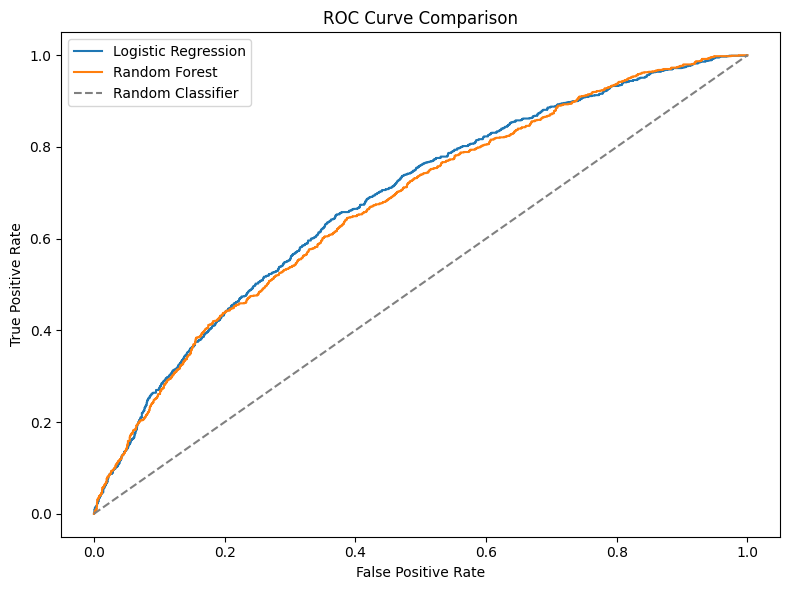
\includegraphics[width=0.8\textwidth]{images/outputroc.png} % Hãy lưu ảnh ROC Curve vào thư mục images với tên này
    \caption{Đường cong ROC so sánh Logistic Regression và Random Forest (Tuned)}
    \label{fig:roc_compare}
\end{figure}

\textit{Nhận xét:} Dựa trên biểu đồ và ROC-AUC, Logistic Regression có khả năng phân tách tổng quát nhỉnh hơn nhẹ so với Random Forest tuned trên tập kiểm thử balanced. Random Forest tuned có Recall lớp nợ xấu cao hơn, nhưng đánh đổi bằng nhiều dự đoán dương tính giả hơn. Vì vậy, Logistic Regression phù hợp hơn làm mô hình triển khai chính trong bối cảnh cần giải thích quyết định tín dụng.
\subsubsection{Đánh giá mức độ quan trọng của Đặc trưng (Feature Importance)}
Một trong những tính năng mạnh mẽ của Random Forest là khả năng trích xuất độ quan trọng của các biến đầu vào. Kết quả (Hình \ref{fig:feature_importance}) cho thấy Top 3 yếu tố quyết định lớn nhất đến khả năng vỡ nợ của một khách hàng bao gồm:
\begin{enumerate}
    \item Lãi suất (\texttt{int\_rate}) - Trọng số: 0.205
    \item Hạng tín dụng (\texttt{grade}) - Trọng số: 0.199
    \item Tỷ lệ nợ trên thu nhập (\texttt{dti\_clipped}) - Trọng số: 0.125
\end{enumerate}

\begin{figure}[H]
    \centering
    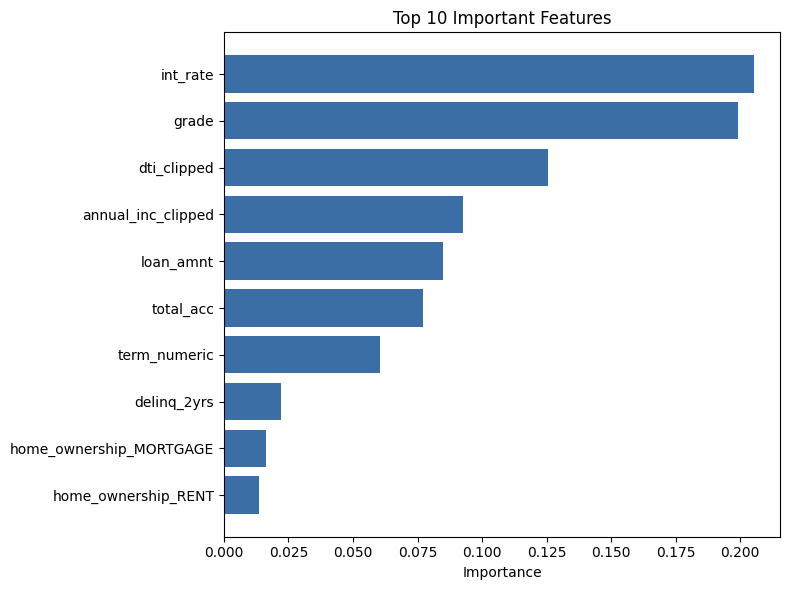
\includegraphics[width=0.8\textwidth]{images/outputfu.png} % Hãy lưu ảnh Feature Importance vào thư mục images với tên này
    \caption{Mức độ quan trọng của các đặc trưng (Top 10 Feature Importance)}
    \label{fig:feature_importance}
\end{figure}

\begin{figure}[H]
    \centering
    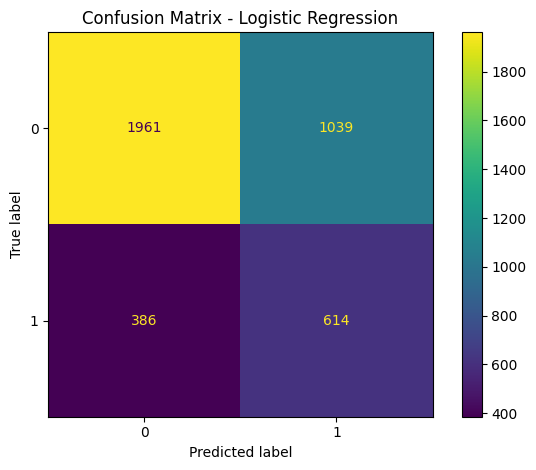
\includegraphics[width=0.8\textwidth]{images/outputcon.png} % Hãy lưu ảnh Confusion Matrix vào thư mục images với tên này
    \caption{Ma trận nhầm lẫn (Confusion Matrix) của Random Forest và Logistic Regression}
    \label{fig:confusion_matrix}
\end{figure}

\subsubsection{Trích xuất và Triển khai Mô hình (Model Export)}
Kết thúc quá trình phân tích, để chuẩn bị cho việc xây dựng ứng dụng hoặc tích hợp vào hệ thống máy chủ, nhóm đã tiến hành đóng gói (serialize) toàn bộ quy trình bằng \texttt{joblib} và \texttt{json}. 

Hệ thống đã lưu trữ thành công các cấu phần cốt lõi tại thư mục \texttt{/app/models/}:
\begin{itemize}
    \item Pipeline mô hình chính: \texttt{loan\_pipeline.pkl} (preprocessing + Logistic Regression).
    \item Mô hình so sánh: \texttt{rf\_tuned\_pipeline.pkl} (preprocessing + Random Forest tuned).
    \item Artifact tương thích: \texttt{lr\_model.pkl} và \texttt{preprocessor\_lr.pkl}.
    \item Cấu hình đặc trưng: \texttt{model\_input\_features.json}, \texttt{feature\_names.json} (25 features sau preprocessing) và \texttt{clip\_params.json}.
\end{itemize}
Bộ hồ sơ triển khai này đảm bảo rằng khi một dòng dữ liệu khách hàng mới (thô) được truyền vào, hệ thống sẽ tự động áp dụng đúng clipping, encoding và scaling đã học từ tập Train trước khi mô hình đưa ra phán quyết cuối cùng.
